\documentclass[paper-main.tex]{subfiles}


\begin{document}


% Optical microphone
% aim of optical microphone: play back injected sounds
A natural successor to simple tomes is complex audio, such as music and speech. 
Complex audio signals are not quasi-monochromatic, unlike continuous gravitational wave signals, so the Viterbi algorithm as implemented in Section~\ref{sec:viterbi_wandering} is not applicable directly.
Instead, in this section, we explore how to use the interferometer as an `optical microphone' to detect and play back complex audio signals, using light to capture sound. 
In doing so, we experiment with a hierarchy of passive filters which suppress noise yet make no assumption about the specific form of the signal, unlike the Fourier-based maximum likelihood matched filter tuned to sinusoidal signals in Section~\ref{sec:single_tone} and Appendix~\ref{app:sinusoid_likelihood} \han{to do}. 
The device has precedence in the laser microphones~\cite{laser_microphone} used in the defence industry which operate on a variety of related principles.
It is also analogous to the detection of unmodelled gravitational-wave signals, e.g. broadband bursts from supernovae~\cite{}\han{to do - add citation}. 
%It is also analogous to the detection of unmodelled gravitational wave signals, e.g. broadband bursts from supernovae. [refs; my last sentence can be improved]


We describe additional components to the demonstration in Section~\ref{sec:photodiode} and initial results in Section~\ref{sec:initialResultsOpMic}.
Filter and speech enhancement techniques applied to the data are detailed in Sections~\ref{sec:simple_filters} and~\ref{sec:logmmse} respectively.
This section is indirectly related to the advanced signal processing required to extract gravitational-wave signals. 
The optical microphone provides an interesting independent demonstration for a broader physics and engineering audience, particularly for the undergraduate lab. 



\subsection{Photodiode}
\label{sec:photodiode}
% advanced method: explain how we capture data

Speech and music recordings require a higher sample rate than that of the webcam ($30\,{\rm Hz}$) used in Sections~\ref{sec:single_tone} and ~\ref{sec:viterbi_wandering}. 
Audible frequencies are in the range $\sim 20\,{\rm Hz}$--$20\,{\rm kHz}$. 
Speech intelligibility requires frequencies up to $3\,{\rm kHz}$ and music requires up to and beyond $8\,{\rm kHz}$~\cite{speech_intelligibility}. 
Therefore the optical microphone data requires a sample rate of at least $16\,{\rm kHz}$ to capture both speech and music. 
We achieved this with a photodiode.


A photodiode is an electrical component that acts as a regular diode when no light is incident on it, blocking any current flow in the `reverse' direction.
As the intensity of incident light rises, it becomes increasingly conductive in the reverse direction. 
% Fundamentally, a current is created in the photodiode by the photo-electric effect.
We place a OSRAM BPW21 photodiode in reverse-bias over an LM358 op-amp. 
This creates a photo-detector that produces a voltage dependent on the incident intensity. 
The photodiode records the interference pattern at roughly the same off-centre position as the webcam in Sections~\ref{sec:single_tone} and~\ref{sec:viterbi_wandering}.
We see no difference when monitoring at other positions in the interference pattern.
The photodiode is mounted on a cloth screen re-purposed from the dismantled commercial speaker, with the electrical leads connected underneath. 


The voltage signal from the photo-detector is captured by a MCP3008 $10$-bit analog-to-digital converter (ADC) connected to a Raspberry Pi Model 3 v1.2~\cite{RaspberryPi:online}, which provides a convenient means to record the photodiode data. 
\han{[from hannah: James does this sound ok? And I have referenced the Raspberry Pi general website, but could you add any appropriate references you used]}
Together, these sample the signal at roughly $16\,{\rm kHz}$.


Sampling any frequency component of the analog signal above the Nyquist frequency of $8\,{\rm kHz}$ leads to aliasing into the detected range. 
To prevent this, we include an anti-aliasing Sallen-Key filter~\cite{sallen_key_filter} tuned to $16\,{\rm kHz}$ before the ADC. 
This component attenuates any frequencies above $8\,{\rm kHz}$, before they are digitally sampled.
We also place another cloth screen over the face of the photodiode, as the reading without it is too high for the ADC after gaining through the op-amps. 
% It’s not clear what limited the sample rate to 16kHz, but it was likely non-optimal reading of the ADC by the Pi script.
% The ADC used (MCP3008) is quoted at 200kHz (or ksps, kilo samples per second).

An updated schematic is shown in Figure~\ref{fig:ifo_schematic_podo} and a photograph of the entire optical microphone in Figure~\ref{fig:setup_pic2}.
See Appendix~\ref{app:circuit_diagram} for a diagram and photograph of the circuit. 


\begin{figure}
	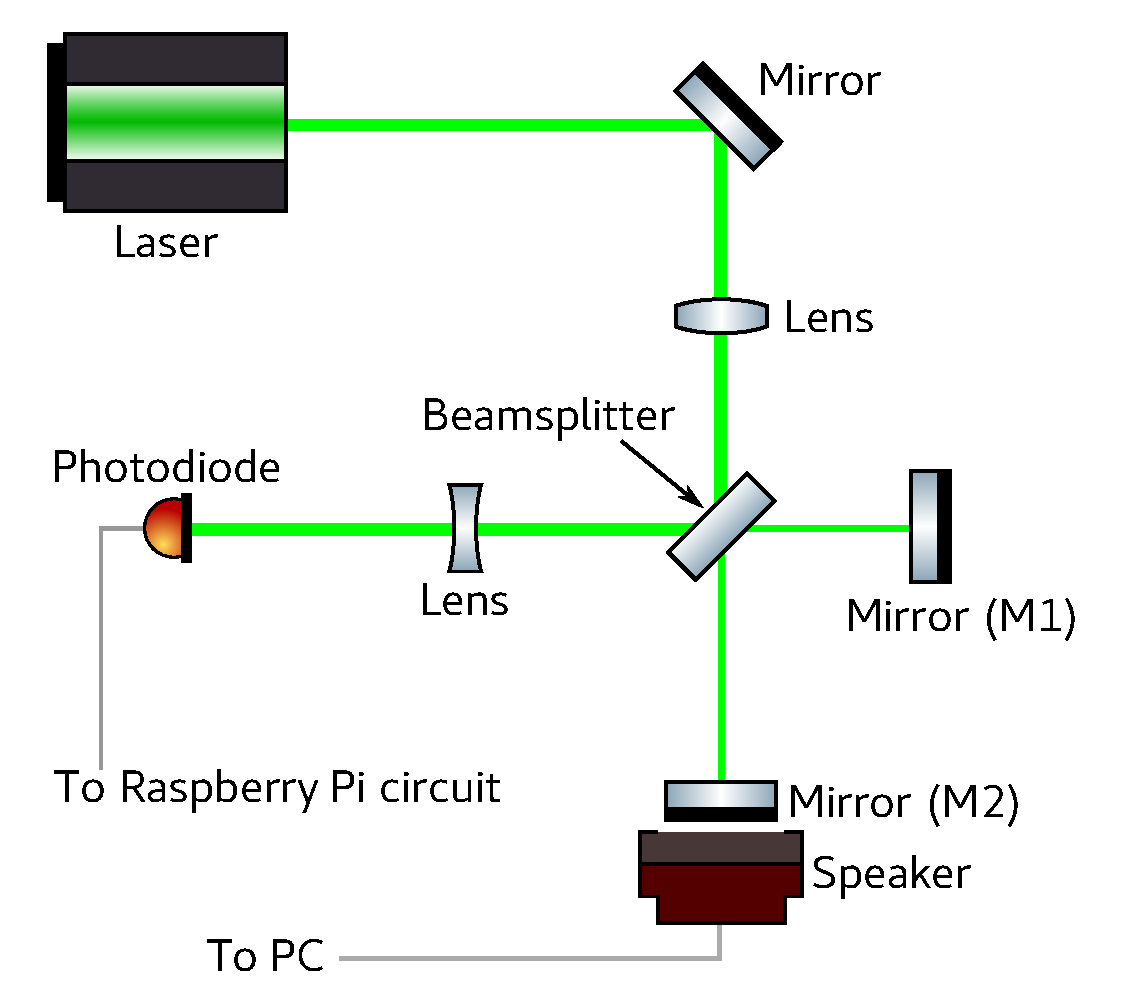
\includegraphics[width=0.49\textwidth]{figures/ifo_schematic_photodiode_edit.pdf}
	\caption{
Michelson interferometer schematic. 
The schematic is identical to Figure~\ref{fig:interference_pattern} except that the data is now recorded using a photodiode and Raspberry Pi instead of a webcam. 
}
	\label{fig:ifo_schematic_podo}
\end{figure}

\begin{figure*}
	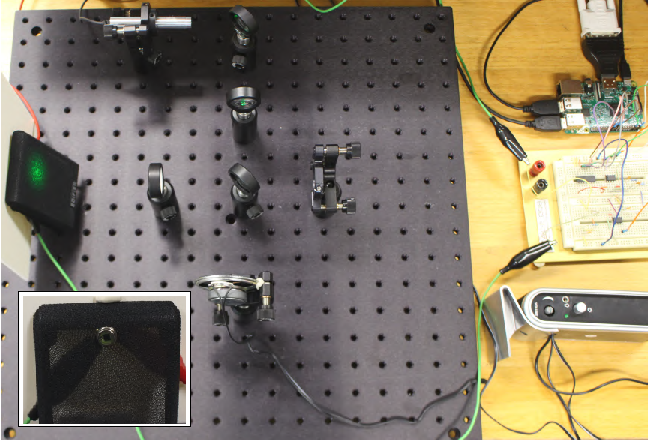
\includegraphics[width=.6\textwidth]{figures/setup_pic2.pdf}
\caption{Photograph of the optical microphone. The Michelson interferometer is shown on the left and the circuit and Raspberry Pi on the right. The interferometer is laid out as in Figure~\ref{fig:ifo_schematic_podo}. In the main image, the photodiode is placed behind the cloth screen. The inset shows a face-on view of the photodiode with the covering screen removed. See Appendix~\ref{app:circuit_diagram} for a circuit diagram and detailed photograph of the circuit.}
	\label{fig:setup_pic2}
\end{figure*}


\subsection{Anti-aliased output}
\label{sec:initialResultsOpMic}
% breakdown of all the filters used along the way
\han{James, if you could rewrite these sentences based on your comments below to reflect exactly what you did, that would be helpful - I don't want to make guesses based on your comments}
The optical microphone is tested on recordings of speech from different people and on music ranging from simple melodies to full track songs. 
Each recording is around one minute long with \jam{processing [this is poor, each recording was functionally ten seconds long, the fact that the sources were minutes long doesn't really matter]} applied to ten second segments. 
For each observation\jam{[again, poor wording, this means that for each 10 s recording we did the following]}, the audio is played through the speaker whilst the Pi script records the signal from the photodiode. 
During recordings, care is taken to ensure minimal activity around the interferometer to reduce environmental noise. 
The timeseries is then directly converted to a .wav file and played as an audio recording using the \textbf{io.wavfile.write} function from the Scipy~\cite{scipy} package in Python~\cite{python} as before.

We find that initial recordings \jam{[Hannah's interpretation is correct here: "We find that the raw output of the optical microphone, collected without special precautions except anti-aliasing, is noisy, with a loud..."?]} are extremely noisy with a loud bass hum throughout.
Each $10\,{\rm s}$ Fourier spectrum shows dominant AC mains noise with power ranging from the fundamental of the $50\,{\rm Hz}$ mains power up to and beyond its $8$th harmonic. \jam{[non-linear appendix, Andrew says to cite Feynman lectures on non-linear oscillations]}
We find that the mains power signal is present in data recorded without an injected audio signal as seen in the power spectral density in Figure~\ref{fig:psd_noise}.
The mains power is also present in data taken with the photodiode in complete darkness with a similar but weaker distribution as that shown in Figure~\ref{fig:psd_noise}).
The origin of the mains power signal is likely to be from the photodiode signal, or environmental noise from the rooms lighting and air conditioning, or a combination. 
\jam{[No idea about the hump at 750 Hz. It is near to the main speech content, but is too broad for me to have any idea]}
\han{[from hannah: okay, perhaps we should just say that we don't know the origin?]}

\begin{figure}
	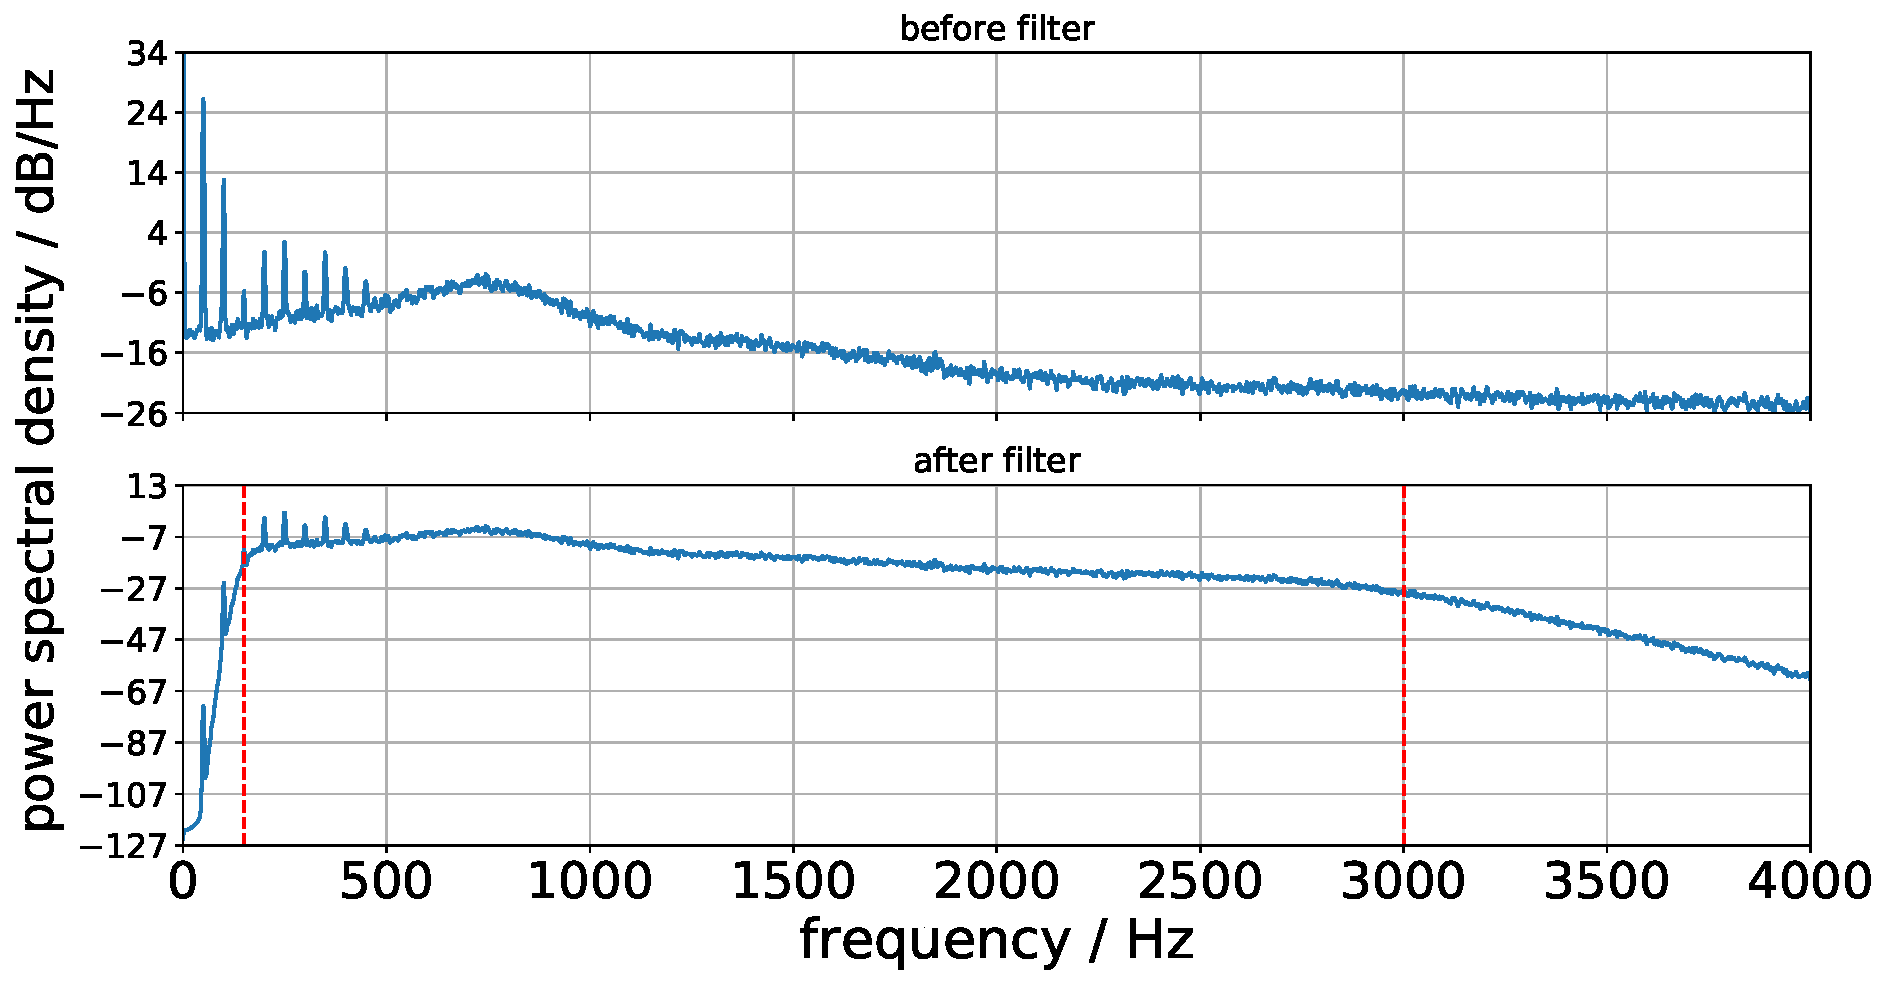
\includegraphics[width=.49\textwidth]{figures/psd_butterworth_14_6.pdf}
	\caption{\label{fig:psd_noise}
Power spectral density (PSD) of background noise (top) from the optical microphone (with the speaker off), and the PSD after applying a Butterworth bandpass filter (bottom) between the two frequencies marked with red, dashed lines. 
We see strong power from the $50\,{\rm Hz}$ mains hum and its harmonics (most likely from the photodiode circuit and the room’s lighting and cooling). Otherwise the PSD is fairly white. 
After filtering we see strong attenuation of all frequencies outside the band, but little change to the harmonics within the band.
}
\end{figure}


\subsection{Additional filters}
\label{sec:simple_filters}

Here we describe several approaches to remove the $50\,{\rm Hz}$ mains hum and its harmonics. 
We test these approaches on $1\,{\rm s}$ of data throughout this section as an illustrative example. 


\begin{figure*}
\begin{center}
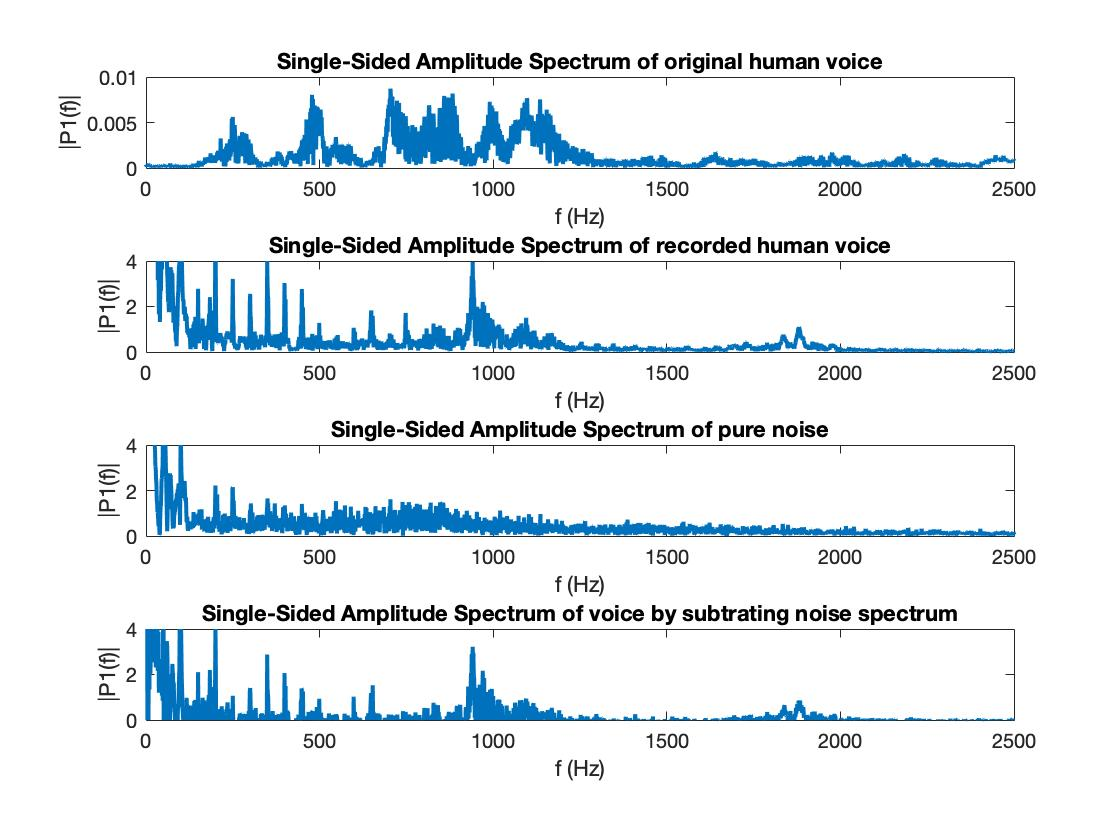
\includegraphics[width=\textwidth]{figures/freqSpectrumOriginalNoiseSubtracted.jpg}
\end{center}
\caption{\label{fig:noiseSubtract}
Frequency spectrum of a $1\,{\rm s}$ signal before the use of filters. 
The first panel shows the original frequency spectrum of the human voice recording (saying ``A cathode ...''). 
The second panel shows the spectrum recorded after the signal passes through the optical microphone (sampled at $16\,000\,{\rm Hz}$).
The third panel shows a noise-only recording from the optical microphone when no audio signal is being played. 
The fourth panel shows the result of subtracting the noise-only spectrum in the third panel from the recording in the second panel. 
We see no obvious improvement from this method. 
}
\end{figure*}

Fig.~\ref{fig:noiseSubtract} shows the frequency spectrum of $1\,{\rm s}$ of recorded speech. 
The first and second panels show the original signal before passing through the interferometer and the optical microphone recording of the signal respectively. 
An intuitive means to remove noise is to subtract the noise spectrum of the instrument directly from the signal spectrum. 
The third panel of Fig.~\ref{fig:noiseSubtract} shows a recording from the optical microphone with no audio signal. 
We see that the output noise is coloured, which reflects the non-linearity of the optical microphone.
The fourth panel of Fig.~\ref{fig:noiseSubtract} shows the frequency spectrum after the noise spectrum has been subtracted. 
We see no obvious improvement, which may be due to time-variant noise. 


The next step is to apply filters to the data. 
The ideal filter would be one that 
\begin{itemize}
\item[i)] completely attenuates the undesired parts of the spectrum, 
\item[ii)] does not change the rest of the spectrum, and 
\item[iii)] has smooth edges so as to not damage the signal after convolution. 
\end{itemize}
These three conditions are contradictory and any filter must compromise between them. 

We note that simply zeroing the frequency channel of each $50\,{\rm Hz}$ in the frequency spectrum is unsuccessful. 
Effectively, this multiplies the spectrum by a rectangular comb filter. 
It does remove the mains harmonics, however it audibly ruins the rest of the signal. 
Applying a filter in frequency space is equivalent to convolving the signal with the inverse Fourier transform of that filter. 
The inverse Fourier transform of a rectangular comb filter (a set of boxcars) is some combination of sinc functions, which significantly corrupt the signal. 

%A smoother comb filter significantly attenuates the spectrum between each harmonic so that the signal is no longer audible. 
\jam{[re:comb filters. When I tried to comb filter it either was too sharp and so jumbled the whole signal in convolution. Or if smooth attenuated the signal away into noise. At least, that's what I remember. Changrong has a comb filter section anyway so I am happy dropping my unsuccessful attempts.]}

Applying a high-pass filter with cut-off frequency $150\,{\rm Hz}$ to the signal works well at removing the $50\,{\rm Hz}$ and $100\,{\rm Hz}$ harmonics.
However, mains harmonics above $100\,{\rm Hz}$ remain. 
The region above $100\,{\rm Hz}$ carries a lot of the fundamental frequencies of speech and music~\cite{speech_intelligibility}. 
Therefore, although a high-pass filter with a higher cut-off removes more harmonics, the played-back signal is unrecognisable. 
Applying a high-pass filter to the logarithm of the signal spectrum does not significantly improve on the above simple high-pass filter.

%We also tried applying a high-pass filter to the logarithm of the signal spectrum and then exponentiating back, but this didn’t significantly improve on the above simple high-pass


\begin{figure}
	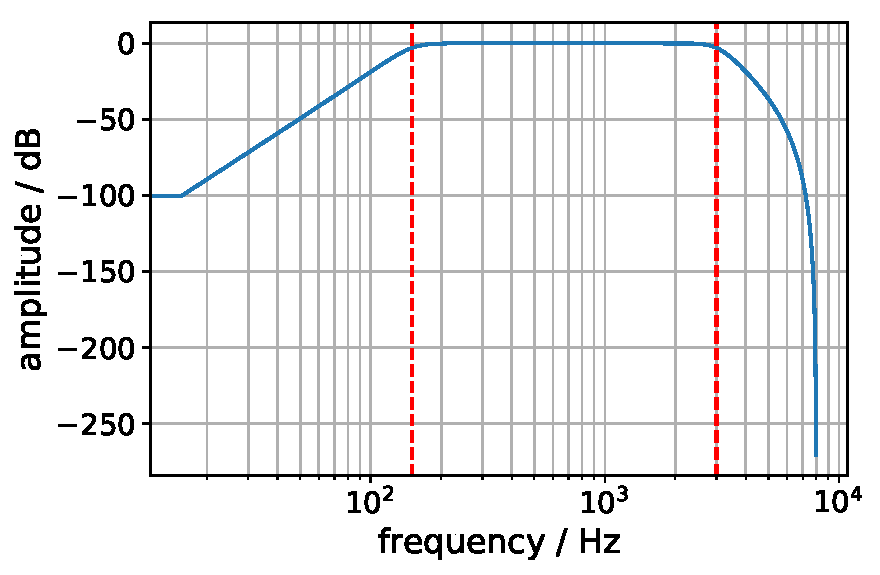
\includegraphics[width=0.49\textwidth]{figures/butterworth_150_3000.pdf}
	\caption{Butterworth bandpass filter frequency response, any amplitude beyond $-3\,{\rm dB}$ is significant attenuation (half power). The red, dashed vertical lines show the band limits of $150\,{\rm Hz}$ and $3\,{\rm kHz}$. Note the flat response within the band.}
	\label{fig:butterworth}
\end{figure}


Band-passing the signal similarly does not address the remaining harmonics above $100\,{\rm Hz}$. 
However, it does suppress other noise at higher frequencies. 
The best performing band-pass filter we find is a fifth order ($n = 5$) Butterworth filter over the range $150\,{\rm Hz}$--$3\,{\rm kHz}$ (beyond $2\,{\rm kHz}$ speech information content drops significantly~\cite{speech_intelligibility}). 
For a low-pass Butterworth filter with cut-off frequency $\omega_c$ and gain $\varepsilon$, the frequency response (attenuation at each frequency) as a function of frequency $\omega$ is:
\begin{equation}
\label{eq:butterworth}
H(\omega) = \left(1+\varepsilon^2 \left( \frac{\omega}{\omega_c} \right)^{2n}\right)^{-\frac{1}{2}}
\end{equation}

\jam{[Andrew wanted a quantitative comment about what the Butterworth does to the PSD, what do I use?]}
To construct a Butterworth band-pass filter, the low-pass filter in Eq.~\ref{eq:butterworth} is combined with a high-pass filter of similar form. 
The response of the filter used is shown in Figure~\ref{fig:butterworth}. 
The Butterworth filter performs the well as it is optimised to be `maximally flat' within the band region (prioritising condition (ii) above).
This filter improves on the above simpler filters but recordings of speech still have low intelligibility.
They can be recognised as speech without being understood.
Looking forward to Sec.~\ref{sec:logmmse}, results for the Butterworth filter are shown in combination with a speech enhancement technique. 

\begin{figure*}
\begin{center}
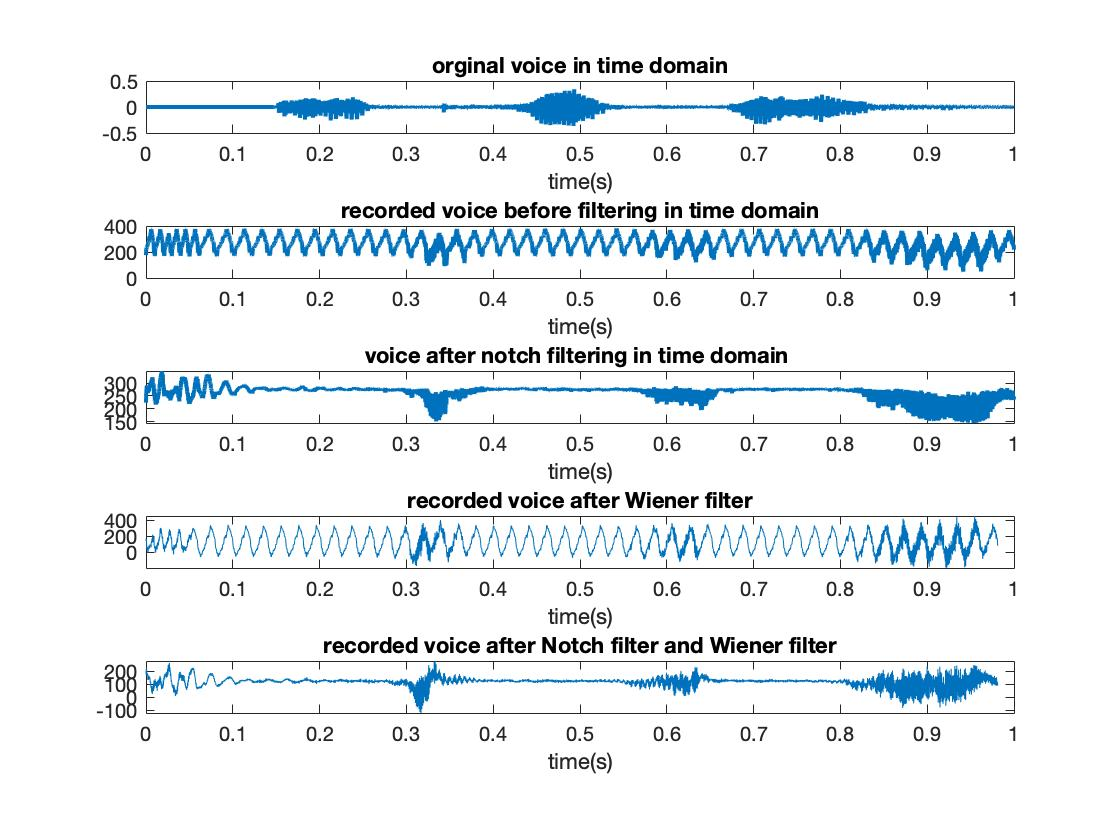
\includegraphics[width=\textwidth]{figures/timeSeriesNotchWiener.jpg}
\end{center}
\caption{\label{fig:timeNotchWiener}
}
\end{figure*}


\begin{figure*}
\begin{center}
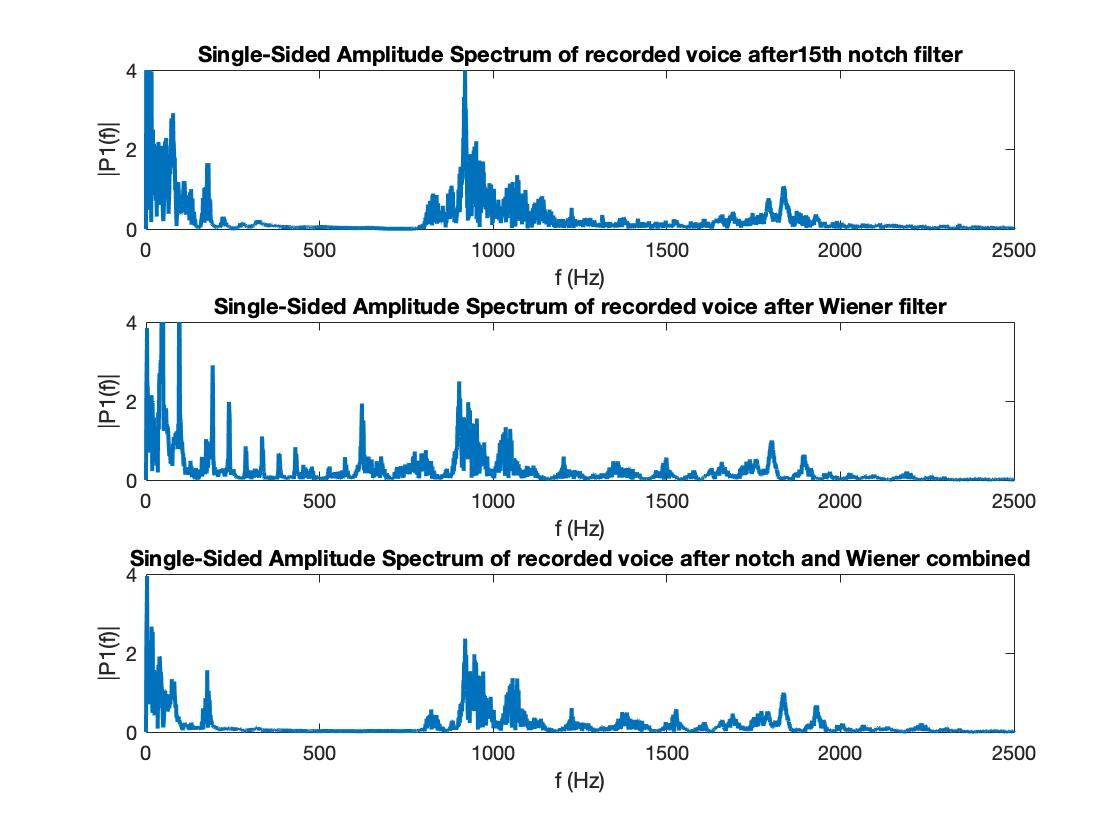
\includegraphics[width=\textwidth]{figures/freqNotchWiener.jpg}
\end{center}
\caption{\label{fig:freqNotchWiener}
}
\end{figure*}

We also consider a combined notch filter and Wiener filter.
Timeseries and frequency spectrum results are shown in Figs.~\ref{fig:timeNotchWiener} and ~\ref{fig:freqNotchWiener} respectively. 
The original signal is identical to that shown in Fig.~\ref{fig:noiseSubtract}.
The first and second panels of Fig.~\ref{fig:timeNotchWiener} show the original audio signal and the recording after passing through the optical microphone (i.e. the timeseries of the data shown in the first two panels of Fig.~\ref{fig:noiseSubtract}). 

A notch filter attenuates signals in specific frequency bands. 
We apply a $15$ cascaded notched filter to remove the mains noise and its harmonics up to $750\,{\rm Hz}$. 
\han{should we include here a mathematical description of the $15$ cascade notch filter?}
\jam{[Yes, I have no idea what a cascaded notched filter is and I'm an author!]}
The timeseries and frequency spectrum results are shown in the third panel of Fig.~\ref{fig:timeNotchWiener} and the first panel of Fig.~\ref{fig:freqNotchWiener}. 
We seen that the mains harmonics are significantly attenuated in comparison to the analysis in Fig.~\ref{fig:noiseSubtract}. 

The Wiener filter produces an estimated signal $\hat{x}$ using linear time-invariant filtering. 
It minimizes the mean square error $\mathbb{E}[(\hat{x}-x)^2]$ between $\hat{x}$ and the actual signal $x$~\citep{verhoeven2009robust}.
\han{should we add more details here too?} \jam{[seconded]}
The timeseries and frequency spectrum results of the Wiener filter are shown in the fourth panel of Fig.~\ref{fig:timeNotchWiener} and the second panel of Fig.~\ref{fig:freqNotchWiener} respectively. 
The timeseries is visibly cleaner, however there is a strong noise hum. 

The combination of the notch filter and the Wiener filter produces a cleaner signal than either individually. 
The time series and spectrum results are shown in the final panels of Figs.~\ref{fig:timeNotchWiener} and ~\ref{fig:freqNotchWiener} respectively.
\han{todo - ask Changrong for some concluding remarks on intelligibility of the result using notch and wiener filter} 

%The ideal filter would be one that i) completely attenuates the undesired parts of the spectrum, ii) does not change the rest of the spectrum, and iii) has smooth edges so as to not damage the signal after convolution. 
%These three conditions are contradictory and any filter must compromise between them. 
%The above simple filters fail one or more of i)--iii). 
%The Butterworth filter performs the best as it is optimised to be `maximally flat' within the band region, prioritising the second condition.
%\han{see note from Andrew and ask James about this}






%\han{Is it worth also including some plots to show how the different filters perform? E.g. a PSD with comb filter, high pass filter, Butterworth filter?}

% Note that we also replicated the Viterbi algorithm results from before with the photodiode, but only with the mains hum removed and high-passing above 100Hz, else the algorithm never selected the signal. Except for being over audible frequencies, there isn’t much difference in the tracking once these filters are applied.


\subsection{logMMSE estimator}
\label{sec:logmmse}
% logMMSE

Speech enhancement for a noisy channel is a classic problem in signal processing. 
Hu~\&~Loizou~(2006)~\cite{SubjectiveComparison} compare 13 speech enhancement methods and find the best to be a log minimum mean-square error (log-MMSE) estimator. 
This type of estimator is based on work by Ephraim~\&~Malah~(1984)~\cite{Ephraim1984SpeechEU_logMMSE} into speech enhancement by minimising the mean square error (MSE) to the logarithm of the spectral (Fourier) amplitude.
The logarithm approximates the response of the human ear~\cite{SubjectiveComparison}.


In this work we use an existing implementation~\cite{logmmse} of the logMMSE estimator. 
Applying this estimator to the optical microphone output produced dramatically cleaner results. 

In Figures~\ref{fig:logMMSE_timeseries} and~\ref{fig:logMMSE_spectrum} we present results from playing a speech recording through the optical microphone. 
Figure~\ref{fig:logMMSE_timeseries} shows the anti-aliased photodiode time series from before (top panel) and after (bottom panel) applying the logMMSE filter. 
Figure~\ref{fig:logMMSE_spectrum} shows the corresponding spectra before (top panel) and after (bottom panel) the logMMSE filter. 
Comparing the before and after spectra shows significant attenuation of all mains harmonics as well as a general smoothing of the spectrum. 

\begin{figure*}
	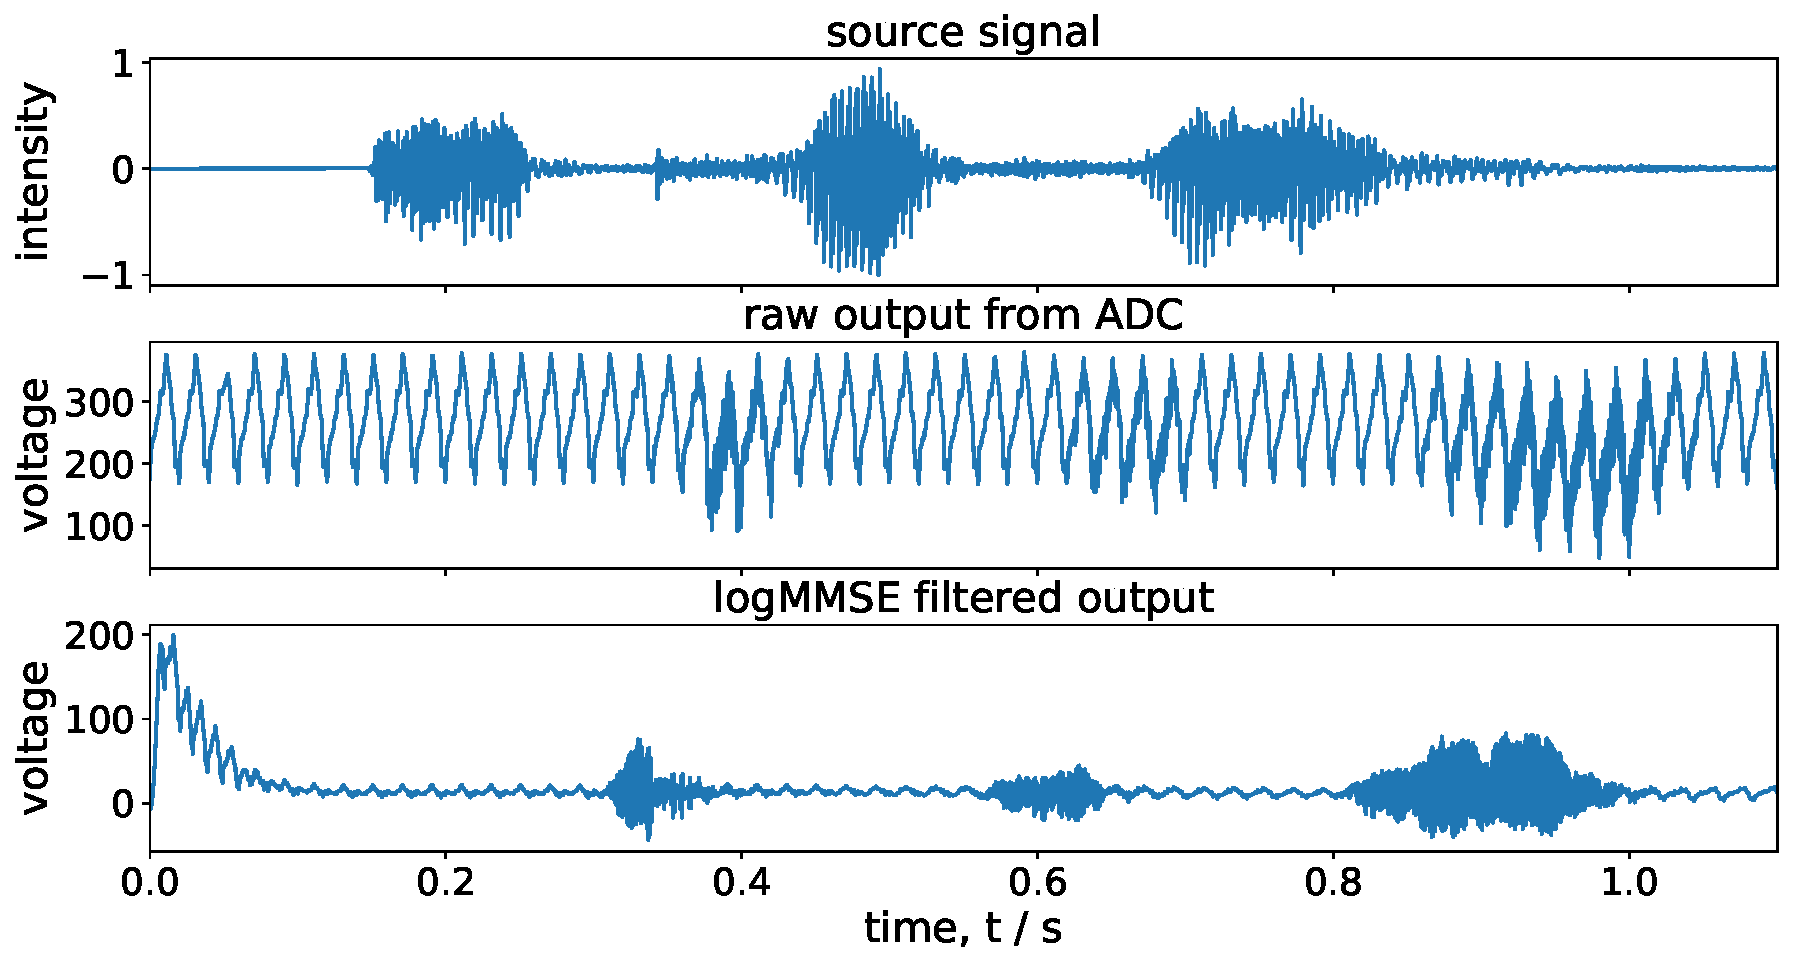
\includegraphics[width=\textwidth]{figures/combined_timeseries_melatos.pdf}
	\caption{Time series of an adult male voice (saying ``A cathode ...'') showing the source (top panel), the optical microphone recording (middle panel), and the recording after filtering with the logMMSE estimator (bottom panel). One second of the one minute recording is shown. The rise at the start of the bottom panel is expected when filtering a signal of finite duration.}
	\label{fig:logMMSE_timeseries}
\end{figure*}

\begin{figure*}
	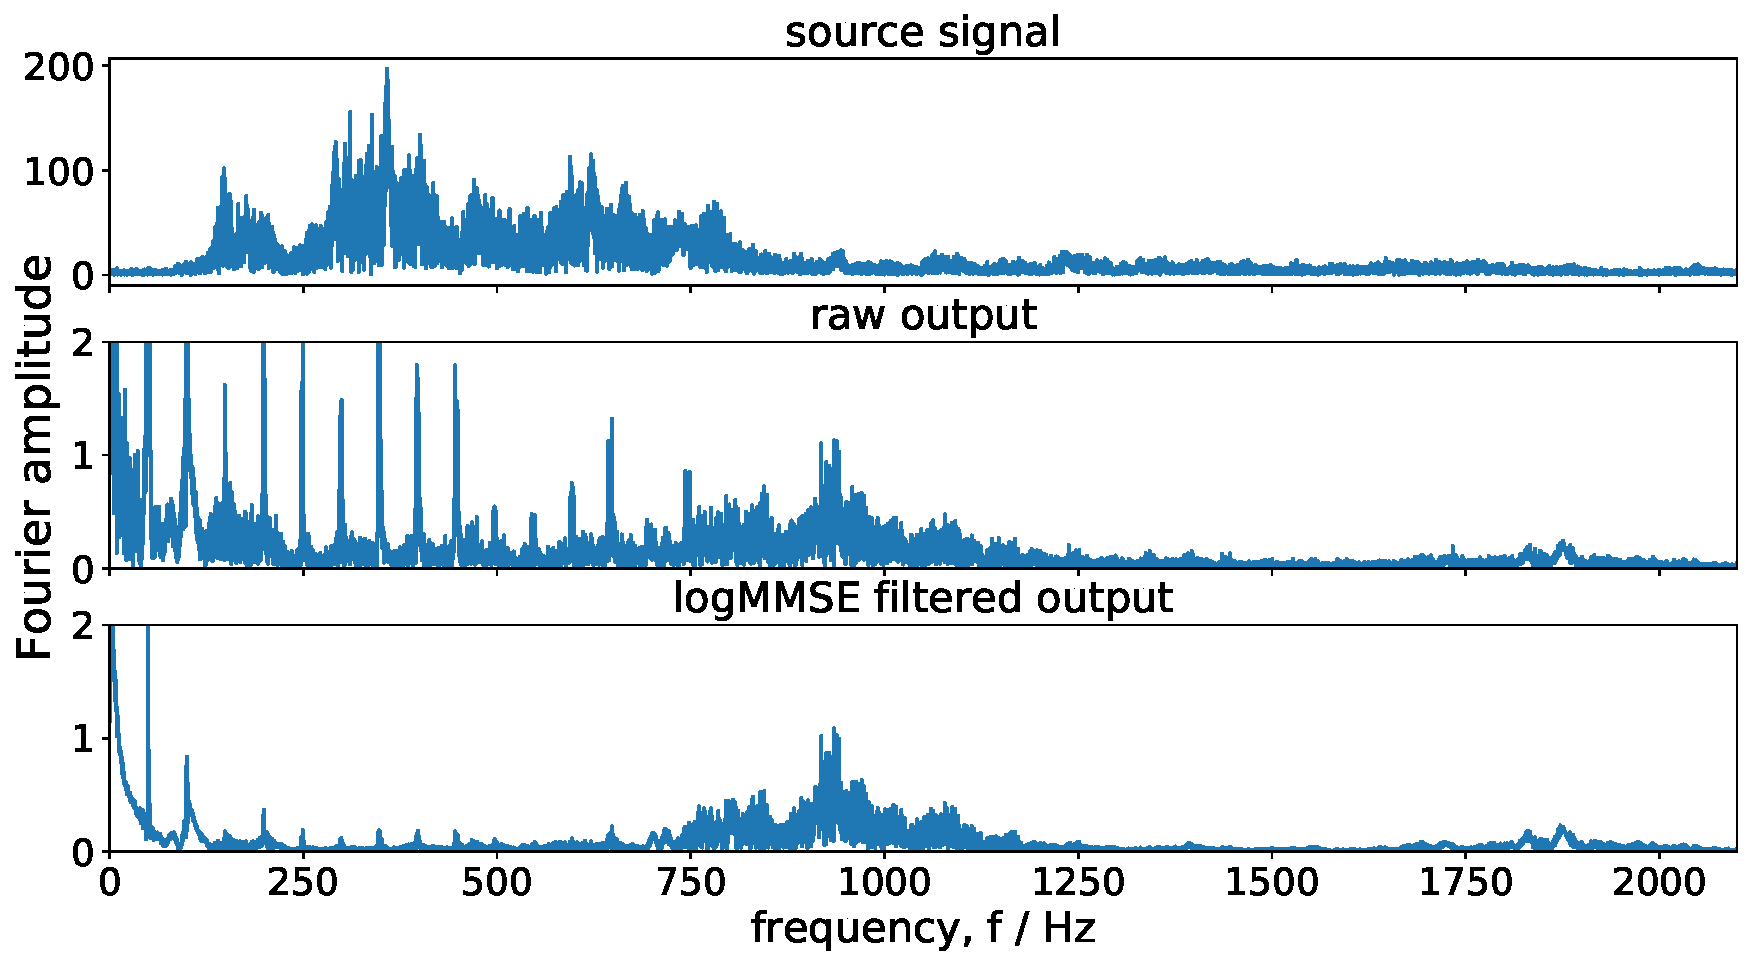
\includegraphics[width=\textwidth]{figures/combined_spectrum_melatos.pdf}
	\caption{Spectrum of optical microphone recording of the same adult male voice in Fig.~\ref{fig:logMMSE_timeseries} showing the source (top panel), the optical microphone recording (middle panel), and the recording after filtering with the logMMSE estimator (bottom panel). The spectrum shows only a detail of the total frequency domain (there is little activity at higher frequencies) and has truncated peaks at amplitude 2 which otherwise dominate the plot.}
	\label{fig:logMMSE_spectrum}
\end{figure*}


We also find improvement with music recordings.
After applying the estimator, simple chords and drums can be heard clearly. 
However more complex melodies are sometimes completely absent. 
From observation, this is especially true for instruments of certain timbres (harmonic profiles), in particular flutes and violins.
This could be a perceptual effect or a frequency dependence somewhere in the optical microphone. 
Speculating, perhaps the speaker-mirror oscillates more at at low frequencies and so instruments like electric bass and drums are louder in the results.


Overall, we find that the intelligibility of speech remains low. 
The played-back voice sounds mumbled and indistinct. 
The estimator removes most of the background noise, but does not clarify the speech. 
To address these problems with the recordings we need to determine whether the signals that are audibly missing (the diction in the speech and complex melodies in music) are indeed being transmitted through the optical microphone at all. 
This requires a better understanding of the system.
% The fringe counting problem of the detector, wherein multiple fringes passing over the array in a single speaker deflection artificially raises the frequency, was noticeable in the speech recordings when compared to the source audio. However, upon comparing injected pure tones, the increase appears to be minimal and inconsistent, at around 5Hz maximum difference. An simple explanation is that the speaker deflections are small compared to manual pressing on the optical table.



\end{document}
